\iffalse
\documentclass[10pt, a4paper]{article}
\usepackage[a4paper,outer=1.5cm,inner=1.5cm,top=1.75cm,bottom=1.5cm]{geometry}

\twocolumn
\usepackage{graphicx}
\usepackage{karnaugh-map}
\usepackage{tabularx}
\usepackage{hyperref}
\usepackage[utf8]{inputenc}
\usepackage{amsmath}
\usepackage{physics}
\usepackage{amssymb}

\begin{document}
\title{Assignment-4}
\author{Name:A.Gowri Priya\and Email :  \url{gowripriyaappayyagari@gmail.com}}
%\{ Wireless Communication (FWC)}
\date{}
\maketitle


  \section{Problem}
  \fi
In  $\triangle  ABC$ and  $\triangle DEF, AB = DE, AB \parallel DE, BC = EF$
and $BC \parallel EF$. Vertices $\vec{A},\vec{B}$ and $\vec{C}$
are joined to
vertices 
$\vec{D},\vec{E}$ and $\vec{F}$
respectively (see Figure 
		\ref{fig:9/8/1/11}
).
Show that
\begin{enumerate}
	\item  quadrilateral  $ABED$ is a parallelogram
	\item  quadrilateral  $BEFC$ is a parallelogram
	\item  $AD \parallel  CF $ and $AD = CF$
		\label{prob:9/8/1/11/3}
	\item  quadrilateral  $ACFD$ is a parallelogram
	\item $AC = DF$
	\item $\triangle ABC \cong \triangle  DEF$.
\end{enumerate}

 	\begin{figure}
		\centering
 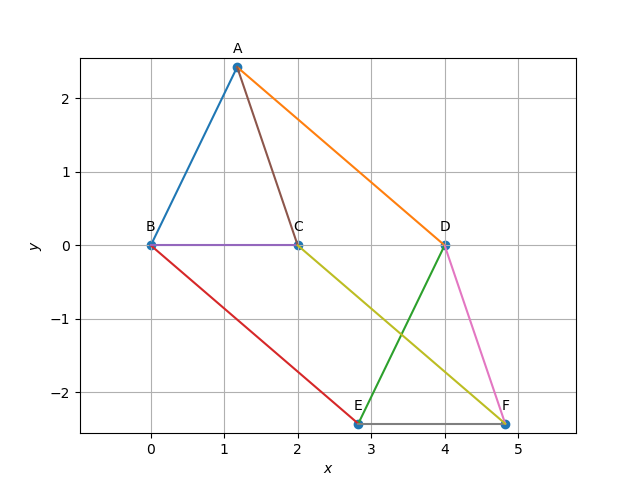
\includegraphics[width=\columnwidth]{chapters/9/8/1/11/figs/fig.png} 
		\caption{}
		\label{fig:9/8/1/11}
  	\end{figure}
\iffalse

\section{Solution}
\begin{center}
The input parameters for this construction are
\begin{tabular}{|c|c|}
	\hline
	\textbf{Symbol}&\textbf{Value}\\
	\hline
	r1&2\\
	\hline
	r2&3\\
	\hline
	$\theta$&$\frac{{3}\pi}{10}$\\
	\hline
\end{tabular}
\boldmath
$$\vec{A}=\begin{pmatrix} r1\cos\theta\\ r2\sin\theta\ \end{pmatrix}$$
$$\vec{B}=\begin{pmatrix} 0\\ 0\ \end{pmatrix}$$
$$\vec{D}=\begin{pmatrix} 4\\ 0\ \end{pmatrix}$$
$$\vec{C}={\vec{B}+\vec{D}}/2$$
$$\vec{E}={\vec{B}+\vec{D}-\vec{A}}$$
$$\vec{F}={\vec{E}+\vec{C}-\vec{B}}$$
\unboldmath
\end{center}
\textbf{Direction vectors}

The Direction vectors are
\boldmath
$$\vec{m_1}={\vec{A}-\vec{B}} $$
$$\vec{m_2}={\vec{B}-\vec{C}} $$
$$\vec{m_3}={\vec{C}-\vec{A}} $$
$$\vec{n_1}={\vec{D}-\vec{E}} $$
$$\vec{n_2}={\vec{E}-\vec{F}} $$
$$\vec{n_3}={\vec{F}-\vec{D}} $$
$$\vec{o_1}={\vec{A}-\vec{D}} $$
$$\vec{o_2}={\vec{C}-\vec{F}} $$
\unboldmath
\textbf{To proove\\ i.Quadrilateral ABED is a parallelogram}\\
\fi
\solution 
From the given information
\begin{align}
		\label{eq:9/8/1/11/1}
	\vec{A}-\vec{B}&= \vec{D}-\vec{E}
	\\
	\vec{B}-\vec{E}&= \vec{C}-\vec{F}
		\label{eq:9/8/1/11/2}
\end{align}
\begin{enumerate}
	\item From Appendix 
	  \ref{eq:two-pgm}, 
		\eqref{eq:9/8/1/11/1} defines the parallelogram $ABED$.
	\item Similarly, 
		\eqref{eq:9/8/1/11/2} defines the parallelogram $BEFC$.
	\item From 
		\eqref{eq:9/8/1/11/1}
		and 
		\eqref{eq:9/8/1/11/2},
\begin{align}
	\vec{A}-\vec{D}=
 \vec{C}-\vec{F}
		\label{eq:9/8/1/11/3}
\end{align}
which  yields
		\ref{prob:9/8/1/11/3}.
	\item 
		\eqref{eq:9/8/1/11/3} implies that $ACFD$ is a parallelogram.
	\item \eqref{eq:9/8/1/11/3} implies $AC = DF$.
	\item Obvious from the fact the $ABCD, BEFC$ and $ACFD$ are parallelograms.
\end{enumerate}
\iffalse

    Distance between A and B is $\norm{\vec{A-B}}$\\
	Distance between D and E is $\norm{\vec{D-E}}$\\
	if $\norm{\vec{A-B}}$ =  $\norm{\vec{D-E}}$\\
	then AB = DE..........(1)\\
	if $\vec{m_1} \times \vec{n_1}=0$\\
	then AB $\parallel$ DE...........(2)\\
	Because,Two vectors ara parallel when cross product of that two vectors is zero.\\
	From (1) and (2) we can say that ABED is a parallelogram.Because,If one pair of opposite sides of a quadrilateral are equal and parallel to each other,then it is a parallelogram.\\
	$\therefore$ Quadrilateral ABED is a parallelogram.\\ 
\textbf{ii.Quadrilateral BEFC is a parallelogram}\\
    Distance between B and C is $\norm{\vec{B-C}}$\\
	Distance between E and F is $\norm{\vec{E-F}}$\\
	if $\norm{\vec{B-C}}$ =  $\norm{\vec{E-F}}$\\
	then BC = EF..........(3)\\
	if $\vec{m_2} \times \vec{n_2}=0$\\
	then BC $\parallel$ EF...........(4)\\
	Because,Two vectors ara parallel when cross product of that two vectors is zero.\\
	From (3) and (4) we can say that BEFC is a parallelogram.Because,If one pair of opposite sides of a quadrilateral are equal and parallel to each other,then it is a parallelogram.\\
	$\therefore$ Quadrilateral BEFC is a parallelogram.\\ 	
\textbf{iii.AD$\parallel$CF and AD=CF}\\
    Distance between A and D is $\norm{\vec{A-D}}$\\
	Distance between C and F is $\norm{\vec{C-F}}$\\
	if $\norm{\vec{A-D}}$ =  $\norm{\vec{C-F}}$\\
	then AD = CF..........(5)\\
	if $\vec{O_1} \times \vec{O_2}=0$\\
	then AD $\parallel$ CF...........(6)\\
	Because,Two vectors ara parallel when cross product of that two vectors is zero.\\
	From (5) and (6) AD$\parallel$CF and AD=CF \\
\textbf{iv.Quadrilateral ACFD is a parallelogram}\\
   From (iii) we can say that AD$\parallel$CF and AD=CF 
	SO, we can say that ACFD is a parallelogram.Because,If one pair of opposite sides of a quadrilateral are equal and parallel to each other,then it is a parallelogram.\\
	$\therefore$ Quadrilateral ACFD is a parallelogram.\\
\textbf{v.AC=DF}\\
    Distance between A and C is $\norm{\vec{A-C}}$\\
	Distance between D and F is $\norm{\vec{D-F}}$\\
	if $\norm{\vec{A-C}}$ =  $\norm{\vec{D-F}}$\\
	then AC = DF\\
	$\therefore$ AC=DF\\
\textbf{vi.$\triangle ABC \cong \triangle DEF$}  \\
If $\norm{\vec{A-B}}$ =  $\norm{\vec{D-E}}$ and $\norm{\vec{B-C}}$ =  $\norm{\vec{E-F}}$ and $\norm{\vec{A-C}}$ =  $\norm{\vec{D-F}}$\\
Then,$\triangle ABC \cong \triangle DEF$ .Because, If three sides of one triangle are equal to three sides of another triangle, the triangles are congruent.(By SSS Rule)\\
$\therefore$ $\triangle ABC \cong \triangle DEF$
\section{Execution}
*Verify the above proofs in the following code.\\
\framebox{
\url{https://github.com/gowripriya-2002/FWC/blob/main/line_assignment/line.py}}	
\bibliographystyle{ieeetr}
\end{document}
\fi
